\documentclass[12pt, a4paper, oneside]{ctexart}
\usepackage{amsmath, amsthm, amssymb, bm, color, framed, graphicx, hyperref, mathrsfs, mathtools, enumerate, tikz}
\usepackage{float}
\usepackage{subcaption} 



\usetikzlibrary{patterns}

\title{\textbf{Homework 4}}
\author{萃英学院\qquad 2022级\qquad 王一鑫}
\date{\today}
\linespread{1.5}
\newcounter{problemname}
\newenvironment{problem}{\begin{framed}\stepcounter{problemname}\par\noindent\textsc{Problem \arabic{problemname}. }}{\end{framed}\par}
\newenvironment{solution}{%
	\par\noindent\textsc{Solution. }\ignorespaces
}{%
	\hfill$\qed$\par
}
\newenvironment{note}{\par\noindent\textsc{Note of Problem \arabic{problemname}. }}{\\\par}

\begin{document}
	
	\maketitle
	
	\begin{problem}
		(Exercise 3.17)

        \begin{enumerate}[(i)]
            \item Find the number of trees on \(n\) vertices in which a given vertex is an end-vertex.
            \item Deduce that, if \(n\) is large, then the probability that a given vertex of a tree 
            with \(n\) vertices is an end-vertex is approximately \(e^{-1}\).
        \end{enumerate}    

	\end{problem}
    
	\begin{solution}
        \begin{enumerate}[(i)]
            \item We start by noting that a leaf must be connected to exactly one other vertex.
        We can choose the neighbor of the leaf in $n - 1$ ways. The remaining $n - 1$
        vertices form a tree, which can be counted using Cayley's formula. 
        The number of trees on $n - 1$ vertices is $(n-1)^{n-3}$.  Multiplying by the
        $n - 1$ ways to attach the leaf, we get the number is $(n-1)^{n-2}$.
            \item To deduce the probability that a given vertex is a leaf for large $n$,
        we divide the number of such trees by the total number of trees on $n$ vertices, 
        which is $n^{n-2}$. The result follows from
        \[ \lim_{n\to\infty} \dfrac{(n-1)^{n-2}}{n^{n-2}} = (1-\dfrac{1}{n})^{n-2} = e^{-1}\]
        \end{enumerate}
	    
		
	\end{solution}
		

		
	
	\begin{problem}
		(Exercise 3.18)

        How many spanning trees has $K_{2,s}$ ?

	\end{problem}
	
	\begin{solution}
		
        Each spanning tree in \( K_{2,s} \) contains one of the two edges \( uv_i \) 
        and \( vw_i \), for each \( i \), together with one extra edge. 
        The number of spanning trees is therefore \( 2^s \times \frac{1}{2}s = s2^{s-1} \).


		
	\end{solution}
	
	\begin{problem}
        (Exercise 3.19)

		Let \(\tau(G)\) be the number of spanning trees in a connected graph \(G\).
        \begin{enumerate}
            \item Prove that, for any edge \(e\), \(\tau(G) = \tau(G - e) + \tau(G \setminus e)\).
            \item Use this result to calculate \(\tau(K_{2,3})\).
        \end{enumerate}

	\end{problem}
	
	\begin{solution}
       
        \begin{enumerate}
            \item Let \( e \) be an edge in \( G \). 
            We consider two cases for spanning trees of \( G \)
            
            If spanning trees do not contain \( e \), then these are exactly 
            the spanning trees of \( G - e \), so there are \( \tau(G - e) \) 
            such trees.

            If spanning trees contain \( e \), contracting \( e \) 
            preserves the tree structure. Each spanning tree of \( G \setminus e \) 
            corresponds uniquely to a spanning tree of \( G \) containing \( e \), 
            so there are \( \tau(G \setminus e) \) such trees.
            
            Since every spanning tree of \( G \) either contains \( e \) or does not, 
            we conclude:
            \[
            \tau(G) = \tau(G - e) + \tau(G \setminus e)
            \]

        
            \item Let \( G = K_{2,3} \). Label the vertices as \( A, B \) 
            in the partition of size 2 and \( 1, 2, 3 \) in the partition of size 3. 
            Choose an edge \( e = A1 \). Apply the formula:
            \[
            \tau(K_{2,3}) = \tau(K_{2,3} - e) + \tau(K_{2,3} \setminus e)
            \]
            
           To compute the first part, remove \( e = A1 \). The remaining edges are \( A2, A3, B1, B2, B3 \). To compute \( \tau(K_{2,3} - e) \), observe that vertex \( A \) must connect via \( A2 \) or \( A3 \), and vertex \( 1 \) must connect via \( B1 \). Applying the formula again by removing edge \( B1 \):
            \[
            \tau(K_{2,3} - e) = \tau((K_{2,3} - e) - B1) + \tau((K_{2,3} - e) \setminus B1)
            \]
            \begin{enumerate}[(i)]
                \item \( (K_{2,3} - e) - B1 \): Removing \( B1 \) disconnects vertex \( 1 \), so \( \tau = 0 \).
                \item \( (K_{2,3} - e) \setminus B1 \): Contract \( B1 \), merging \( B \) and \( 1 \) into \( B' \). The resulting graph \( G' \) has edges \( A2, A3, B'2, B'3 \), which is \( K_{2,2} \). Thus, \( \tau(G') = 2 \times 2 = 4 \).
            \end{enumerate}
            Hence, \( \tau(K_{2,3} - e) = 0 + 4 = 4 \).
            
            Now contract \( e = A1 \), merging \( A \) and \( 1 \) into \( A' \). The contracted graph \( G'' \) has vertices \( A', B, 2, 3 \) with edges \( A'2, A'3, BA', B2, B3 \). Apply the formula by removing edge \( BA' \):
            \[
            \tau(G'') = \tau(G'' - BA') + \tau(G'' \setminus BA')
            \]
            \begin{enumerate}[(i)]
                \item \( G'' - BA' \): The graph becomes $K_{2,2}$.
                \item \( G'' \setminus BA' \): Contract \( BA' \), merging \( B \) and \( A' \) into \( B'' \). The resulting graph has edges \( B''2, B''3 \) (twice each). The number of spanning trees is \( 2 \times 2 = 4 \).
            \end{enumerate}
            Hence, \( \tau(G'') = 4 + 4 = 8 \). Finally,
            \[
            \tau(K_{2,3}) = \tau(K_{2,3} - e) + \tau(K_{2,3} \setminus e) = 4 + 8 = 12
            \]
            
            Therefore, \( \tau(K_{2,3}) = 12 \).
        \end{enumerate}
		
	\end{solution}
	
	
	
	\begin{problem}
        (Exercise 3.21) 
        
        Find a minimum weight spanning tree in the graph in Fig.\ref{fig:3.21}.
        \begin{figure}[H]
			\small
			\centering
			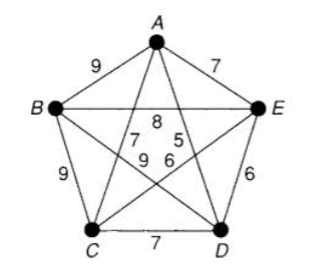
\includegraphics[width=0.5\columnwidth]{figure/fig1.png}
			\caption{Figure For Problem 4}
			\label{fig:3.21}
		\end{figure}
		
	\end{problem}
	
	\begin{solution}
        By applying greedy algorithm we obtain the minimum weight spanning tree in the graph
        is shown in Fig \ref{fig:mw}. And the minimum weight is $25$.
		\begin{figure}[H]
			\small
			\centering
			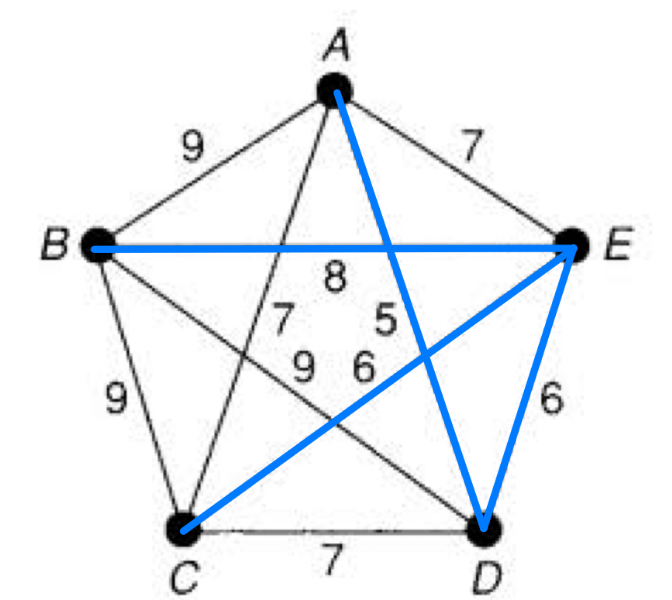
\includegraphics[width=0.5\columnwidth]{figure/fig6.jpg}
			\caption{Solution For Problem 4}
			\label{fig:mw}
		\end{figure}
		
	\end{solution}


	\begin{problem}
		(Exercise 3.23)

        \begin{enumerate}[(i)]
            \item How would you adapt the greedy algorithm to find a \textit{maximum} weight spanning tree?
            \item Find a maximum weight spanning tree for each of the weighted graphs in Figs \ref{fig:3.15} and \ref{fig:3.28}.
        \end{enumerate}
        

		\begin{figure}[H]
            \centering
            \begin{minipage}{0.49\linewidth}
                \centering
                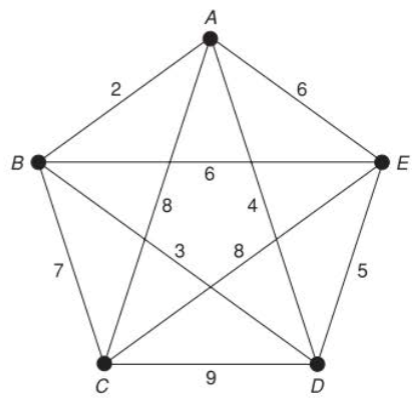
\includegraphics[width=0.7\linewidth]{figure/fig2.png}
                \caption{Weighted Graph 1}
                \label{fig:3.15}
            \end{minipage}
            %\qquad
            \begin{minipage}{0.49\linewidth}
                \centering
                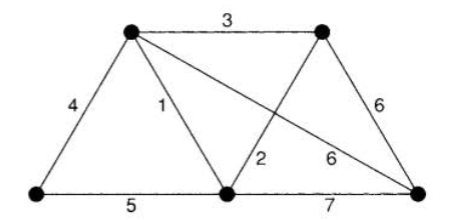
\includegraphics[width=0.9\linewidth]{figure/fig3.png}
                \caption{Weighted Graph 2}
                \label{fig:3.28}
            \end{minipage}
        \end{figure}
        
		
    \end{problem}

	\begin{solution}
        \begin{enumerate}[(i)]
            \item We can adapt the algorithm by chossing $e_k$ as the edge
            of  largest weight in the graph at each stage.
            \item The maximum weight spanning tree for each of the weighted
            graphs is shown in Fig \ref{mw1} and \ref{mw2}.
            \begin{figure}[H]
                \centering
                \begin{minipage}{0.49\linewidth}
                    \centering
                    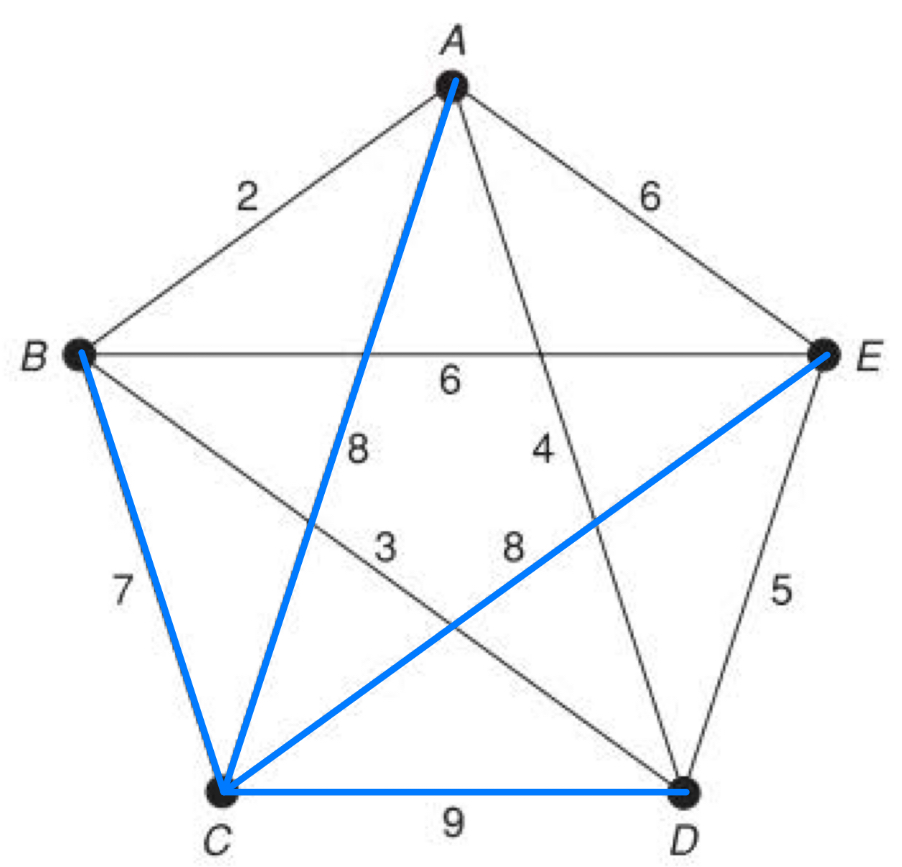
\includegraphics[width=0.7\linewidth]{figure/fig7.jpg}
                    \caption{Maximum Weighted Graph 1}
                    \label{mw1}
                \end{minipage}
                %\qquad
                \begin{minipage}{0.49\linewidth}
                    \centering
                    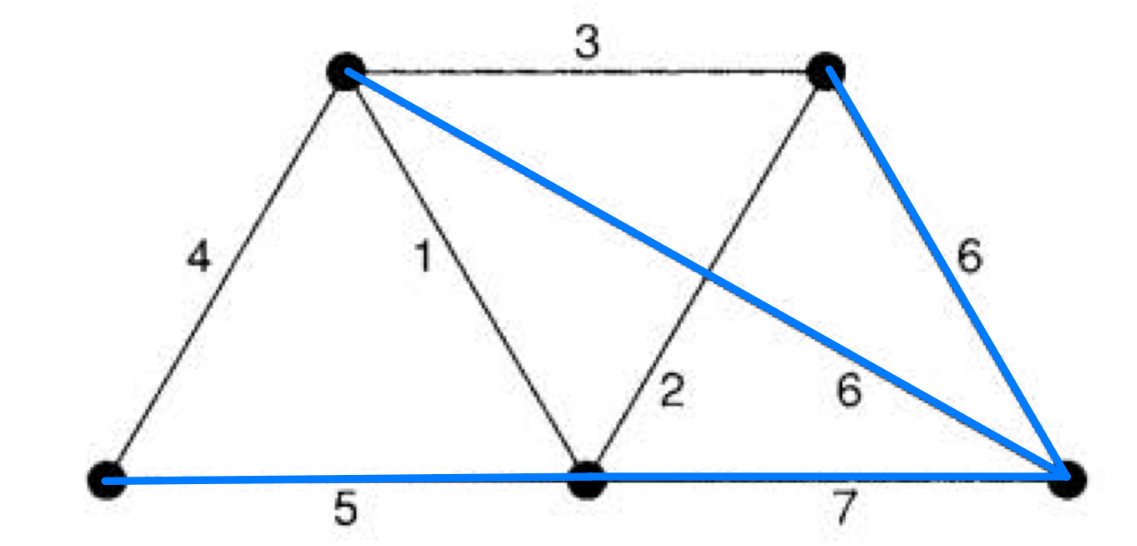
\includegraphics[width=0.9\linewidth]{figure/fig8.jpg}
                    \caption{Maximum Weighted Graph 2}
                    \label{mw2}
                \end{minipage}
            \end{figure}
        \end{enumerate}
		Moreover, the maximum weighted is $32$ and $24$ respectively.

    \end{solution}
		
    
	\begin{problem}
		(Exercise 3.26)

        Perform a breadth-first search and a depth-first search on the tree in Fig. \ref{fig:3.31}
        \begin{figure}[H]
			\small
			\centering
			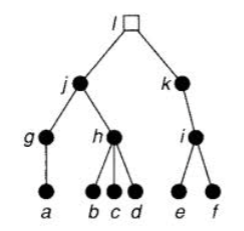
\includegraphics[width=0.32\columnwidth]{figure/fig4.png}
			\caption{Figure For Problem 6}
			\label{fig:3.31}
		\end{figure}
        

    \end{problem}

	\begin{solution}
		It is directly from definition.
        \begin{figure}[H]
			\small
			\centering
			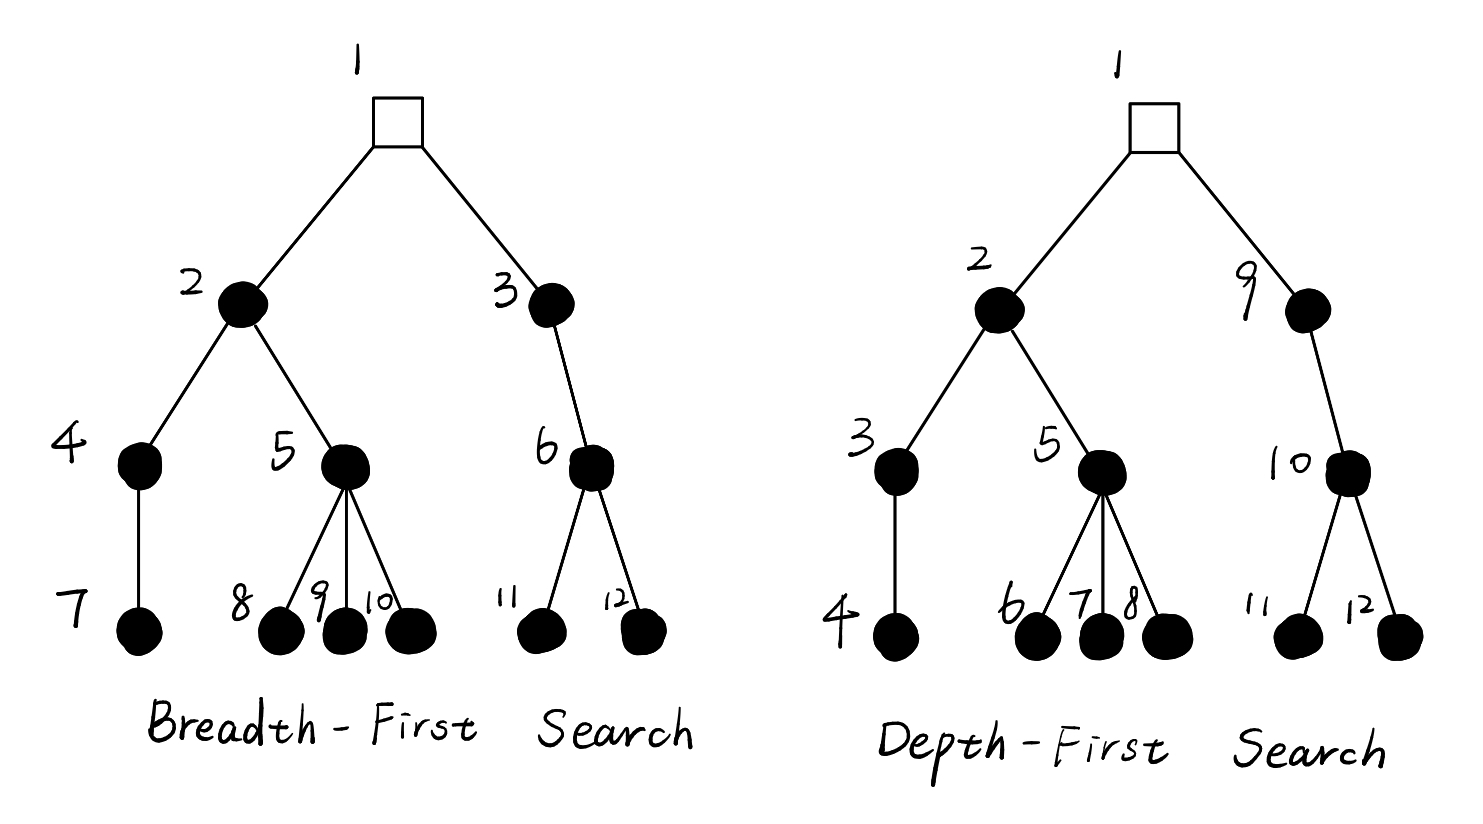
\includegraphics[width=0.9\columnwidth]{figure/fig9.jpg}
			\caption{Solution For Problem 6}
			\label{fig:search}
		\end{figure}
		
		
	\end{solution}


	\begin{problem}
		
        Determine whether the braced framework in Fig. \ref{fig:3.33} is rigid, and whether the bracing is a minimum bracing.
        \begin{figure}[H]
			\small
			\centering
			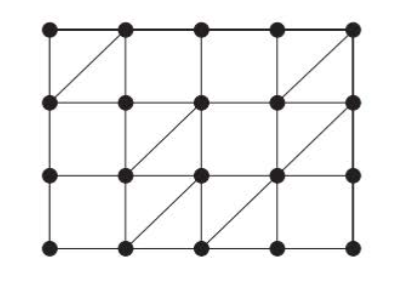
\includegraphics[width=0.5\columnwidth]{figure/fig5.png}
			\caption{Figure For Problem 7}
			\label{fig:3.33}
		\end{figure}

	\end{problem}

	\begin{solution}

    We can draw the corresponding bipartite as Fig \ref{fig:bi}.
    \begin{figure}[H]
        \small
        \centering
        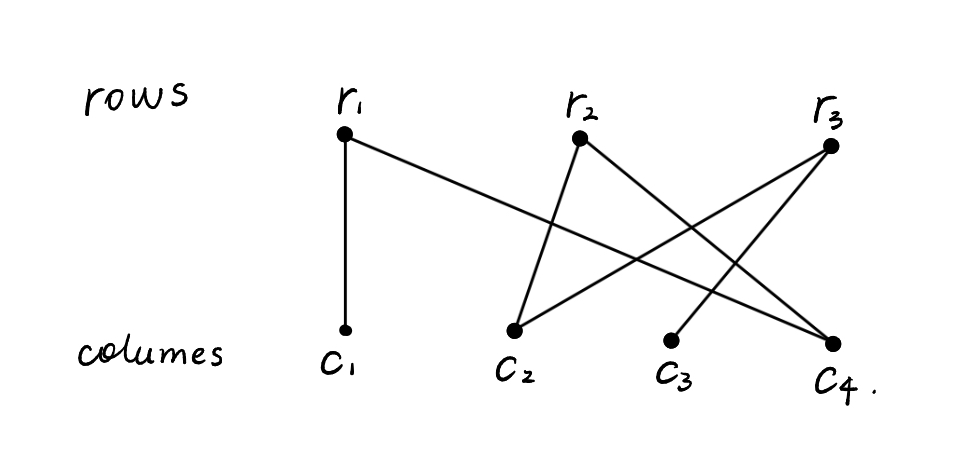
\includegraphics[width=0.8\columnwidth]{figure/fig10.jpg}
        \caption{bipartite}
        \label{fig:bi}
    \end{figure}
    We can find that the bipartite is connected, thus the braced framework is rigid.
    Moreover, since it contains no cycles and has $6$ edges, it is a tree, thus the
    bracing is a minimum bracing.
	\end{solution}
     

    \begin{problem}
        (Exercise 3.32)

        \begin{enumerate}[(i)]
            \item Let $C^*$ be a set of edges of a connected graph $G$. Show that, if $C^*$ has an edge in common with each spanning tree of $G$, then $C^*$ contains a cutset.
            \item Obtain a corresponding result for cycles.
        \end{enumerate}
        
    \end{problem}
	
    \begin{solution}
        \begin{enumerate}[(i)]
            \item Assume \( C^* \) intersects every spanning tree of \( G \). 
        Then, the complement of \( C^* \) , denoted as \( E(G) \setminus C^* \),
        cannot contain any spanning tree, as spanning trees must include 
        at least one edge from \( C^* \). Therefore, \( G - C^* \) 
        (the graph obtained by removing \( C^* \)) is disconnected. 
        By definition, a cutset is a minimal set of edges whose removal 
        disconnects the graph. Since \( C^* \) disconnects \( G \), 
        it must contain at least one minimal such set, i.e., a cutset. 
        Hence, \( C^* \) contains a cutset.
            \item Suppose \( D^* \) intersects every cotree (the complement of spanning trees). 
            Assume for contradiction that \( D^* \) contains no cycle. 
            Then \( D^* \) is a forest (a union of trees). 
            A forest can be extended to a spanning tree \( T \). 
            The cotree \( E(G) \setminus T \) would then be disjoint 
            from \( D^* \), contradicting the assumption that \( D^* \) 
            intersects every cotree. Thus, \( D^* \) must contain 
            at least one cycle.

        \end{enumerate}
        



    \end{solution}
\end{document}


